\documentclass[12pt]{article}
\usepackage{geometry}
    \geometry{
        a4paper,
        lmargin=2cm,
        rmargin=2cm,
        tmargin=2cm,
        bmargin=2cm
    }
\usepackage{float}
\usepackage{indentfirst}
\usepackage{caption}
\usepackage{graphicx}
\usepackage{fontspec}
\usepackage{listings}
\usepackage{color}
\usepackage[T1]{fontenc}
\lstloadlanguages{C,C++,csh,Java}

\setmainfont[Mapping=tex-text]{Times New Roman}
\definecolor{red}{rgb}{0.6,0,0}
\definecolor{blue}{rgb}{0,0,0.6}
\definecolor{green}{rgb}{0,0.8,0}
\definecolor{cyan}{rgb}{0.0,0.6,0.6}
\renewcommand{\contentsname}{Sadržaj}

\title{Domaći 5 - OPC UA}
\author{Ognjen Čavić E2 161/2024}
\date{Decembar 2024}
\begin{document}
\maketitle
\section{Opis Problema}
\par U sistem je potrebno dodati još jedan tip motora koji proizvodi firma Rade
Končar.
Potom je potrebno dodati da se u metodu pokretanja sistema njegova brzina
postavi na nulu i potrebno je napraviti još jednu metodu koja omogućava proizvoljno
menjanje brzine tog motora.
\section{Logika rešenja}
\par U \textbf{XML} datoteku koja opisuje \textbf{OPC} server dodaje se novi tip
motora \textbf{RadeKončarMotorType} koji je izveden iz klase
\textbf{GenericMotorType} i kao takav se dodaje pokretnoj traci.
Dodavanje metode za podešavanje brzine zahteva definisanje posebnog tipa metoda
\textbf{changeMotorSpeedMethodType} koji zahteva jedan ulazni argument i posle
se taj tip instancira na istom mestu kao i druge dve metode.
\par U kodu, unutar \textbf{BatchPlantManager} klase se modifikuju metode
\textbf{OnStartProcess} i \textbf{OnStopProcess} tako da uključuju (postavljaju
brzinu na nulu) i isključuju (postavljaju brzinu na -1) motor, respektivno.
Dodaje se i metoda \textbf{OnChangeMotorSpeed} koja služi za postavljanje
brzine motora na osnovu argumenta.
Ukoliko motor nije uključen pri pozivu ove metode ili ukoliko je zadata brzina
vrednost koja je izvan opsega, metoda vraća odgovarajuću grešku.
Poslednje što preostaje je da se u metodi \textbf{CreateAddressSpace} povežu
metode iz klase sa onim na serveru koji je opisan u \textbf{XML} fajlu.
Takođe je u ovoj metodi i brzina motora postavljena na -1, čisto da na početku
vrednost brzine ne bi bila \textbf{NULL}.
\section{Rezultati}
\begin{center}
	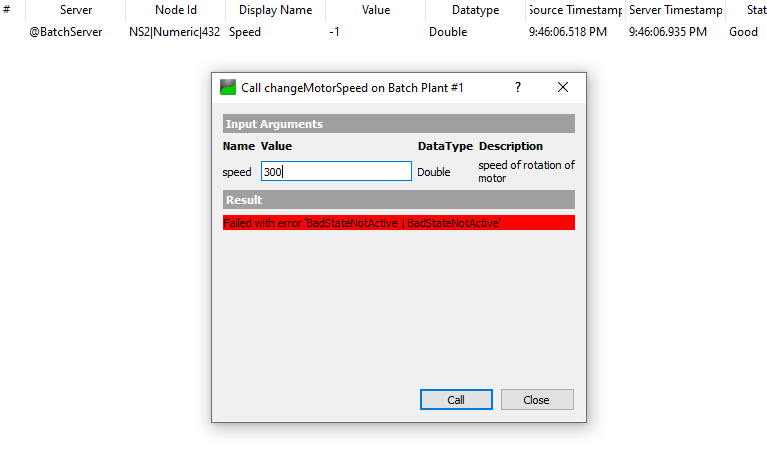
\includegraphics[scale=0.7]{figs/menjanjeBrzineIskljMotora.PNG}
	\captionof*{figure}{Slika 1: Pokušaj postavljanja brzine kada je motor
	isključen}
\end{center}
\vspace{0.5cm}
\begin{center}
	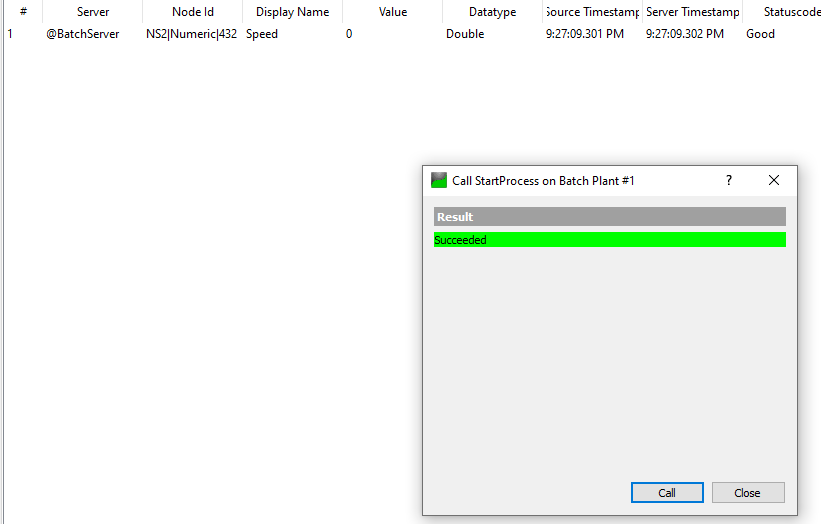
\includegraphics[scale=0.7]{figs/ukljucenMotor.PNG}
	\captionof*{figure}{Slika 2: Uključivanje motora}
\end{center}
\begin{center}
	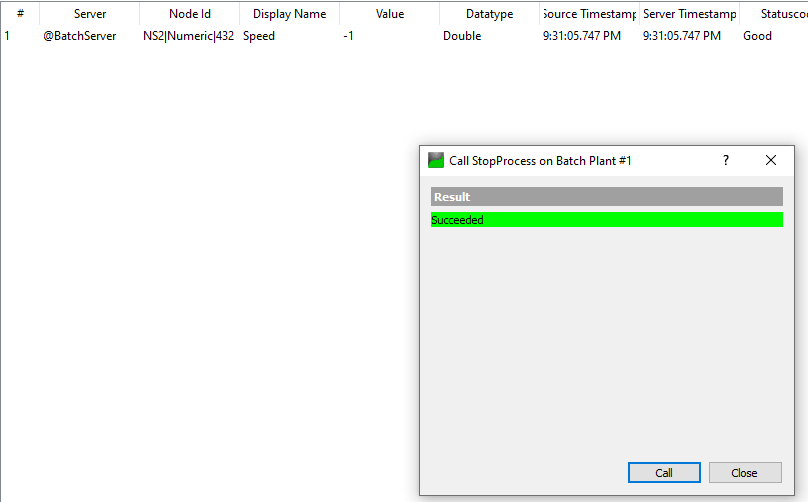
\includegraphics[scale=0.7]{figs/gasenjeMotora.PNG}
	\captionof*{figure}{Slika 3: Iskljucivanje motora}
\end{center}
\vspace{2cm}
\begin{center}
	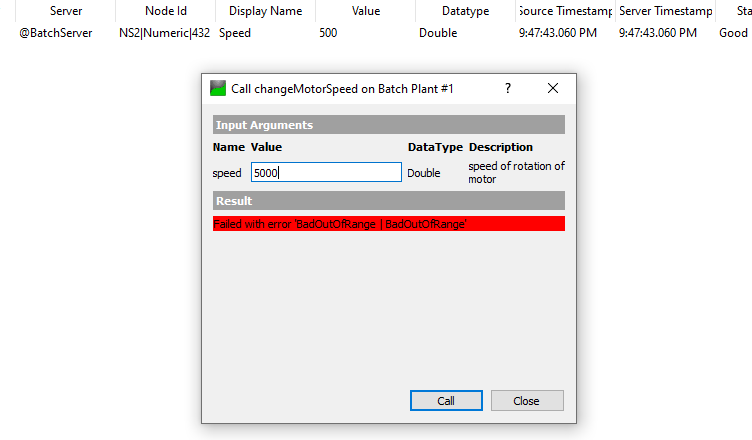
\includegraphics[scale=0.7]{figs/brzinaMotoraVanOpsega.PNG}
	\captionof*{figure}{Slika 4: Pokušaj zadavanja brzine izvan opsega}
\end{center}
\end{document}
